\documentclass[11pt,aspectratio=169]{beamer}
% =============================================================================
%  Shared Beamer preamble — Machine Learning I & II, PEU-CD 2026 (ENEI / INEI)
%
%  Inherited from the ML_Foundations deck (Alexander Quispe), with three changes:
%    * `minted` removed — it shells out to Pygments and does not build under
%      tectonic; every code block in the course uses `listings`.
%    * unused packages (lipsum, blindtext, multimedia, videoframe) dropped.
%    * `bbm` dropped — its fonts are PK-only and tectonic cannot render them;
%      the indicator uses \mathbf{1} instead.
%    * a math-macro block added so all twelve lectures share one notation.
%
%  Each lecture is a standalone document:
%      \documentclass[11pt,aspectratio=169]{beamer}
%      % =============================================================================
%  Shared Beamer preamble — Machine Learning I & II, PEU-CD 2026 (ENEI / INEI)
%
%  Inherited from the ML_Foundations deck (Alexander Quispe), with three changes:
%    * `minted` removed — it shells out to Pygments and does not build under
%      tectonic; every code block in the course uses `listings`.
%    * unused packages (lipsum, blindtext, multimedia, videoframe) dropped.
%    * `bbm` dropped — its fonts are PK-only and tectonic cannot render them;
%      the indicator uses \mathbf{1} instead.
%    * a math-macro block added so all twelve lectures share one notation.
%
%  Each lecture is a standalone document:
%      \documentclass[11pt,aspectratio=169]{beamer}
%      % =============================================================================
%  Shared Beamer preamble — Machine Learning I & II, PEU-CD 2026 (ENEI / INEI)
%
%  Inherited from the ML_Foundations deck (Alexander Quispe), with three changes:
%    * `minted` removed — it shells out to Pygments and does not build under
%      tectonic; every code block in the course uses `listings`.
%    * unused packages (lipsum, blindtext, multimedia, videoframe) dropped.
%    * `bbm` dropped — its fonts are PK-only and tectonic cannot render them;
%      the indicator uses \mathbf{1} instead.
%    * a math-macro block added so all twelve lectures share one notation.
%
%  Each lecture is a standalone document:
%      \documentclass[11pt,aspectratio=169]{beamer}
%      \input{../../../style/preamble}
% =============================================================================

% ---------- fonts ----------
\usepackage{helvet}
\usepackage[default]{lato}
\usepackage{tgbonum}
\usepackage{mathpazo}
\usepackage[utf8]{inputenc}

% ---------- math ----------
\usepackage{amsmath,amssymb}
\usepackage{mathtools}

% ---------- graphics, tables, layout ----------
\usepackage{graphicx}
\usepackage{tikz}
\usetikzlibrary{positioning,calc,arrows,arrows.meta,decorations.markings,shapes.misc,matrix,shapes,fit}
\usepackage{array}
\usepackage{booktabs}
\usepackage{multirow}
\usepackage{dcolumn}
\usepackage{subcaption}
\usepackage{caption}
\usepackage{changepage}
\usepackage{xspace}
\usepackage{tcolorbox}
\tcbuselibrary{skins,breakable}
\usepackage[ruled,vlined]{algorithm2e}
\usepackage{listings}
\usepackage{appendixnumberbeamer}
\usepackage{hyperref}

\newcolumntype{d}[0]{D{.}{.}{5}}
\setbeamertemplate{caption}[numbered]

% ---------- palette (Okabe–Ito, colour-blind safe) ----------
\definecolor{blue}{RGB}{0,114,178}
\definecolor{red}{RGB}{213,94,0}
\definecolor{yellow}{RGB}{240,228,66}
\definecolor{green}{RGB}{0,158,115}
\definecolor{MyBackground}{RGB}{255,253,218}

\hypersetup{colorlinks=true, linkbordercolor={white}, linkcolor={blue}, urlcolor={blue}}

% ---------- beamer look ----------
\setbeamercolor{frametitle}{fg=blue}
\setbeamercolor{title}{fg=black}
\setbeamertemplate{footline}[frame number]
\setbeamertemplate{navigation symbols}{}
\setbeamertemplate{itemize items}{-}
\setbeamercolor{itemize item}{fg=blue}
\setbeamercolor{itemize subitem}{fg=blue}
\setbeamercolor{enumerate item}{fg=blue}
\setbeamercolor{enumerate subitem}{fg=blue}
\setbeamercolor{button}{bg=MyBackground,fg=blue}
\setbeamercolor{section in toc}{fg=blue}
\setbeamercolor{subsection in toc}{fg=red}
\setbeamersize{text margin left=1em,text margin right=1em}
\setbeamercolor{block title}{fg=white,bg=blue}
\setbeamercolor{block body}{bg=blue!5}
\setbeamercolor{block title alerted}{fg=white,bg=red}
\setbeamercolor{block body alerted}{bg=red!5}
\setbeamercolor{block title example}{fg=white,bg=green}
\setbeamercolor{block body example}{bg=green!5}
\setbeamertemplate{blocks}[rounded][shadow=false]

\newenvironment{wideitemize}{\itemize\addtolength{\itemsep}{10pt}}{\enditemize}

\newenvironment{transitionframe}{
  \setbeamercolor{background canvas}{bg=yellow}
  \begin{frame}}{
  \end{frame}
}

% Section divider: a plain frame with a large blue title.
\newcommand{\sectionframe}[1]{%
  \section{#1}%
  \begin{frame}[plain]\vfill\begin{center}{\Huge\textcolor{blue}{#1}}\end{center}\vfill\end{frame}}

% ---------- proof / derivation environments ----------
% derivation: a boxed, step-by-step algebraic argument. Title is the claim.
\newtcolorbox{derivation}[1]{enhanced, colback=blue!3, colframe=blue, fonttitle=\bfseries,
  title={#1}, boxrule=0.6pt, left=4pt, right=4pt, top=3pt, bottom=3pt, arc=2pt}
% claim: a result to be proved (theorem / lemma / proposition).
\newtcolorbox{claim}[1]{enhanced, colback=white, colframe=black, fonttitle=\bfseries,
  title={#1}, boxrule=0.6pt, left=4pt, right=4pt, top=3pt, bottom=3pt, arc=2pt}
% keypoint: the one line to remember from a slide.
\newtcolorbox{keypoint}{enhanced, colback=green!6, colframe=green, boxrule=0.6pt,
  left=4pt, right=4pt, top=3pt, bottom=3pt, arc=2pt}
% caution: a common mistake or a subtlety.
\newtcolorbox{caution}{enhanced, colback=red!5, colframe=red, boxrule=0.6pt,
  left=4pt, right=4pt, top=3pt, bottom=3pt, arc=2pt}

% ---------- code ----------
\lstset{
  basicstyle=\ttfamily\scriptsize, keywordstyle=\color{blue}\bfseries,
  commentstyle=\color{green}, stringstyle=\color{red},
  showstringspaces=false, breaklines=true, frame=single, rulecolor=\color{black!30},
  numbers=none, xleftmargin=4pt, framexleftmargin=4pt, language=Python
}

\input{../../../style/macros}

% ---------- course-wide title metadata ----------
\newcommand{\courseinstitution}{ENEI -- INEI \,\textperiodcentered\, PEU-CD 2026}
\newcommand{\courseauthor}{Alexander Quispe}
\institute{\courseinstitution}
\author{\courseauthor}

% =============================================================================

% ---------- fonts ----------
\usepackage{helvet}
\usepackage[default]{lato}
\usepackage{tgbonum}
\usepackage{mathpazo}
\usepackage[utf8]{inputenc}

% ---------- math ----------
\usepackage{amsmath,amssymb}
\usepackage{mathtools}

% ---------- graphics, tables, layout ----------
\usepackage{graphicx}
\usepackage{tikz}
\usetikzlibrary{positioning,calc,arrows,arrows.meta,decorations.markings,shapes.misc,matrix,shapes,fit}
\usepackage{array}
\usepackage{booktabs}
\usepackage{multirow}
\usepackage{dcolumn}
\usepackage{subcaption}
\usepackage{caption}
\usepackage{changepage}
\usepackage{xspace}
\usepackage{tcolorbox}
\tcbuselibrary{skins,breakable}
\usepackage[ruled,vlined]{algorithm2e}
\usepackage{listings}
\usepackage{appendixnumberbeamer}
\usepackage{hyperref}

\newcolumntype{d}[0]{D{.}{.}{5}}
\setbeamertemplate{caption}[numbered]

% ---------- palette (Okabe–Ito, colour-blind safe) ----------
\definecolor{blue}{RGB}{0,114,178}
\definecolor{red}{RGB}{213,94,0}
\definecolor{yellow}{RGB}{240,228,66}
\definecolor{green}{RGB}{0,158,115}
\definecolor{MyBackground}{RGB}{255,253,218}

\hypersetup{colorlinks=true, linkbordercolor={white}, linkcolor={blue}, urlcolor={blue}}

% ---------- beamer look ----------
\setbeamercolor{frametitle}{fg=blue}
\setbeamercolor{title}{fg=black}
\setbeamertemplate{footline}[frame number]
\setbeamertemplate{navigation symbols}{}
\setbeamertemplate{itemize items}{-}
\setbeamercolor{itemize item}{fg=blue}
\setbeamercolor{itemize subitem}{fg=blue}
\setbeamercolor{enumerate item}{fg=blue}
\setbeamercolor{enumerate subitem}{fg=blue}
\setbeamercolor{button}{bg=MyBackground,fg=blue}
\setbeamercolor{section in toc}{fg=blue}
\setbeamercolor{subsection in toc}{fg=red}
\setbeamersize{text margin left=1em,text margin right=1em}
\setbeamercolor{block title}{fg=white,bg=blue}
\setbeamercolor{block body}{bg=blue!5}
\setbeamercolor{block title alerted}{fg=white,bg=red}
\setbeamercolor{block body alerted}{bg=red!5}
\setbeamercolor{block title example}{fg=white,bg=green}
\setbeamercolor{block body example}{bg=green!5}
\setbeamertemplate{blocks}[rounded][shadow=false]

\newenvironment{wideitemize}{\itemize\addtolength{\itemsep}{10pt}}{\enditemize}

\newenvironment{transitionframe}{
  \setbeamercolor{background canvas}{bg=yellow}
  \begin{frame}}{
  \end{frame}
}

% Section divider: a plain frame with a large blue title.
\newcommand{\sectionframe}[1]{%
  \section{#1}%
  \begin{frame}[plain]\vfill\begin{center}{\Huge\textcolor{blue}{#1}}\end{center}\vfill\end{frame}}

% ---------- proof / derivation environments ----------
% derivation: a boxed, step-by-step algebraic argument. Title is the claim.
\newtcolorbox{derivation}[1]{enhanced, colback=blue!3, colframe=blue, fonttitle=\bfseries,
  title={#1}, boxrule=0.6pt, left=4pt, right=4pt, top=3pt, bottom=3pt, arc=2pt}
% claim: a result to be proved (theorem / lemma / proposition).
\newtcolorbox{claim}[1]{enhanced, colback=white, colframe=black, fonttitle=\bfseries,
  title={#1}, boxrule=0.6pt, left=4pt, right=4pt, top=3pt, bottom=3pt, arc=2pt}
% keypoint: the one line to remember from a slide.
\newtcolorbox{keypoint}{enhanced, colback=green!6, colframe=green, boxrule=0.6pt,
  left=4pt, right=4pt, top=3pt, bottom=3pt, arc=2pt}
% caution: a common mistake or a subtlety.
\newtcolorbox{caution}{enhanced, colback=red!5, colframe=red, boxrule=0.6pt,
  left=4pt, right=4pt, top=3pt, bottom=3pt, arc=2pt}

% ---------- code ----------
\lstset{
  basicstyle=\ttfamily\scriptsize, keywordstyle=\color{blue}\bfseries,
  commentstyle=\color{green}, stringstyle=\color{red},
  showstringspaces=false, breaklines=true, frame=single, rulecolor=\color{black!30},
  numbers=none, xleftmargin=4pt, framexleftmargin=4pt, language=Python
}

% =============================================================================
%  Notation — one convention for all lectures
%
%  scalars      x, y, w           plain italic
%  vectors      \vx \vy \vw       bold lower-case
%  matrices     \vX \vW \vSigma   bold upper-case
%  parameters   \vbeta \vtheta    bold Greek
%  transpose    \vX\T             \top
% =============================================================================
\newcommand{\R}{\mathbb{R}}
\newcommand{\E}{\mathbb{E}}
\newcommand{\Prob}{\mathbb{P}}
\DeclareMathOperator{\Var}{Var}
\DeclareMathOperator{\Cov}{Cov}
\DeclareMathOperator{\tr}{tr}
\DeclareMathOperator{\diag}{diag}
\DeclareMathOperator{\rank}{rank}
\DeclareMathOperator{\sign}{sign}
\DeclareMathOperator{\col}{col}
\DeclareMathOperator{\RSS}{RSS}
\DeclareMathOperator*{\argmin}{arg\,min}
\DeclareMathOperator*{\argmax}{arg\,max}
\newcommand{\norm}[1]{\left\lVert #1 \right\rVert}
\newcommand{\abs}[1]{\left\lvert #1 \right\rvert}
\newcommand{\inner}[2]{\left\langle #1,\, #2 \right\rangle}
\newcommand{\ind}[1]{\mathbf{1}\!\left\{#1\right\}}
\newcommand{\T}{^{\top}}
\newcommand{\inv}{^{-1}}
\newcommand{\half}{\tfrac{1}{2}}
\newcommand{\eps}{\varepsilon}
\newcommand{\Dset}{\mathcal{D}}
\newcommand{\Hset}{\mathcal{H}}
\newcommand{\Lcal}{\mathcal{L}}
\newcommand{\Ncal}{\mathcal{N}}

% bold vectors
\newcommand{\vx}{\mathbf{x}}   \newcommand{\vy}{\mathbf{y}}   \newcommand{\vz}{\mathbf{z}}
\newcommand{\vw}{\mathbf{w}}   \newcommand{\vu}{\mathbf{u}}   \newcommand{\vv}{\mathbf{v}}
\newcommand{\vb}{\mathbf{b}}   \newcommand{\vh}{\mathbf{h}}   \newcommand{\vr}{\mathbf{r}}
\newcommand{\vc}{\mathbf{c}}   \newcommand{\vf}{\mathbf{f}}   \newcommand{\vg}{\mathbf{g}}
\newcommand{\vp}{\mathbf{p}}   \newcommand{\vq}{\mathbf{q}}   \newcommand{\vs}{\mathbf{s}}
\newcommand{\va}{\mathbf{a}}   \newcommand{\vd}{\mathbf{d}}   \newcommand{\vt}{\mathbf{t}}
\newcommand{\vk}{\mathbf{k}}   \newcommand{\vm}{\mathbf{m}}   \newcommand{\vn}{\mathbf{n}}
\newcommand{\vzero}{\mathbf{0}} \newcommand{\vone}{\mathbf{1}}
% bold matrices
\newcommand{\vX}{\mathbf{X}}   \newcommand{\vY}{\mathbf{Y}}   \newcommand{\vZ}{\mathbf{Z}}
\newcommand{\vW}{\mathbf{W}}   \newcommand{\vH}{\mathbf{H}}   \newcommand{\vI}{\mathbf{I}}
\newcommand{\vA}{\mathbf{A}}   \newcommand{\vB}{\mathbf{B}}   \newcommand{\vC}{\mathbf{C}}
\newcommand{\vD}{\mathbf{D}}   \newcommand{\vP}{\mathbf{P}}   \newcommand{\vQ}{\mathbf{Q}}
\newcommand{\vU}{\mathbf{U}}   \newcommand{\vV}{\mathbf{V}}   \newcommand{\vS}{\mathbf{S}}
\newcommand{\vM}{\mathbf{M}}   \newcommand{\vK}{\mathbf{K}}   \newcommand{\vG}{\mathbf{G}}
% bold Greek
\newcommand{\vbeta}{\boldsymbol{\beta}}     \newcommand{\valpha}{\boldsymbol{\alpha}}
\newcommand{\vtheta}{\boldsymbol{\theta}}   \newcommand{\vmu}{\boldsymbol{\mu}}
\newcommand{\vSigma}{\boldsymbol{\Sigma}}   \newcommand{\vLambda}{\boldsymbol{\Lambda}}
\newcommand{\veps}{\boldsymbol{\varepsilon}} \newcommand{\vphi}{\boldsymbol{\phi}}
\newcommand{\vgamma}{\boldsymbol{\gamma}}   \newcommand{\vlambda}{\boldsymbol{\lambda}}
\newcommand{\vdelta}{\boldsymbol{\delta}}   \newcommand{\vnu}{\boldsymbol{\nu}}
\newcommand{\vxi}{\boldsymbol{\xi}}         \newcommand{\vpi}{\boldsymbol{\pi}}
\newcommand{\vomega}{\boldsymbol{\omega}}



% ---------- course-wide title metadata ----------
\newcommand{\courseinstitution}{ENEI -- INEI \,\textperiodcentered\, PEU-CD 2026}
\newcommand{\courseauthor}{Alexander Quispe}
\institute{\courseinstitution}
\author{\courseauthor}

% =============================================================================

% ---------- fonts ----------
\usepackage{helvet}
\usepackage[default]{lato}
\usepackage{tgbonum}
\usepackage{mathpazo}
\usepackage[utf8]{inputenc}

% ---------- math ----------
\usepackage{amsmath,amssymb}
\usepackage{mathtools}

% ---------- graphics, tables, layout ----------
\usepackage{graphicx}
\usepackage{tikz}
\usetikzlibrary{positioning,calc,arrows,arrows.meta,decorations.markings,shapes.misc,matrix,shapes,fit}
\usepackage{array}
\usepackage{booktabs}
\usepackage{multirow}
\usepackage{dcolumn}
\usepackage{subcaption}
\usepackage{caption}
\usepackage{changepage}
\usepackage{xspace}
\usepackage{tcolorbox}
\tcbuselibrary{skins,breakable}
\usepackage[ruled,vlined]{algorithm2e}
\usepackage{listings}
\usepackage{appendixnumberbeamer}
\usepackage{hyperref}

\newcolumntype{d}[0]{D{.}{.}{5}}
\setbeamertemplate{caption}[numbered]

% ---------- palette (Okabe–Ito, colour-blind safe) ----------
\definecolor{blue}{RGB}{0,114,178}
\definecolor{red}{RGB}{213,94,0}
\definecolor{yellow}{RGB}{240,228,66}
\definecolor{green}{RGB}{0,158,115}
\definecolor{MyBackground}{RGB}{255,253,218}

\hypersetup{colorlinks=true, linkbordercolor={white}, linkcolor={blue}, urlcolor={blue}}

% ---------- beamer look ----------
\setbeamercolor{frametitle}{fg=blue}
\setbeamercolor{title}{fg=black}
\setbeamertemplate{footline}[frame number]
\setbeamertemplate{navigation symbols}{}
\setbeamertemplate{itemize items}{-}
\setbeamercolor{itemize item}{fg=blue}
\setbeamercolor{itemize subitem}{fg=blue}
\setbeamercolor{enumerate item}{fg=blue}
\setbeamercolor{enumerate subitem}{fg=blue}
\setbeamercolor{button}{bg=MyBackground,fg=blue}
\setbeamercolor{section in toc}{fg=blue}
\setbeamercolor{subsection in toc}{fg=red}
\setbeamersize{text margin left=1em,text margin right=1em}
\setbeamercolor{block title}{fg=white,bg=blue}
\setbeamercolor{block body}{bg=blue!5}
\setbeamercolor{block title alerted}{fg=white,bg=red}
\setbeamercolor{block body alerted}{bg=red!5}
\setbeamercolor{block title example}{fg=white,bg=green}
\setbeamercolor{block body example}{bg=green!5}
\setbeamertemplate{blocks}[rounded][shadow=false]

\newenvironment{wideitemize}{\itemize\addtolength{\itemsep}{10pt}}{\enditemize}

\newenvironment{transitionframe}{
  \setbeamercolor{background canvas}{bg=yellow}
  \begin{frame}}{
  \end{frame}
}

% Section divider: a plain frame with a large blue title.
\newcommand{\sectionframe}[1]{%
  \section{#1}%
  \begin{frame}[plain]\vfill\begin{center}{\Huge\textcolor{blue}{#1}}\end{center}\vfill\end{frame}}

% ---------- proof / derivation environments ----------
% derivation: a boxed, step-by-step algebraic argument. Title is the claim.
\newtcolorbox{derivation}[1]{enhanced, colback=blue!3, colframe=blue, fonttitle=\bfseries,
  title={#1}, boxrule=0.6pt, left=4pt, right=4pt, top=3pt, bottom=3pt, arc=2pt}
% claim: a result to be proved (theorem / lemma / proposition).
\newtcolorbox{claim}[1]{enhanced, colback=white, colframe=black, fonttitle=\bfseries,
  title={#1}, boxrule=0.6pt, left=4pt, right=4pt, top=3pt, bottom=3pt, arc=2pt}
% keypoint: the one line to remember from a slide.
\newtcolorbox{keypoint}{enhanced, colback=green!6, colframe=green, boxrule=0.6pt,
  left=4pt, right=4pt, top=3pt, bottom=3pt, arc=2pt}
% caution: a common mistake or a subtlety.
\newtcolorbox{caution}{enhanced, colback=red!5, colframe=red, boxrule=0.6pt,
  left=4pt, right=4pt, top=3pt, bottom=3pt, arc=2pt}

% ---------- code ----------
\lstset{
  basicstyle=\ttfamily\scriptsize, keywordstyle=\color{blue}\bfseries,
  commentstyle=\color{green}, stringstyle=\color{red},
  showstringspaces=false, breaklines=true, frame=single, rulecolor=\color{black!30},
  numbers=none, xleftmargin=4pt, framexleftmargin=4pt, language=Python
}

% =============================================================================
%  Notation — one convention for all lectures
%
%  scalars      x, y, w           plain italic
%  vectors      \vx \vy \vw       bold lower-case
%  matrices     \vX \vW \vSigma   bold upper-case
%  parameters   \vbeta \vtheta    bold Greek
%  transpose    \vX\T             \top
% =============================================================================
\newcommand{\R}{\mathbb{R}}
\newcommand{\E}{\mathbb{E}}
\newcommand{\Prob}{\mathbb{P}}
\DeclareMathOperator{\Var}{Var}
\DeclareMathOperator{\Cov}{Cov}
\DeclareMathOperator{\tr}{tr}
\DeclareMathOperator{\diag}{diag}
\DeclareMathOperator{\rank}{rank}
\DeclareMathOperator{\sign}{sign}
\DeclareMathOperator{\col}{col}
\DeclareMathOperator{\RSS}{RSS}
\DeclareMathOperator*{\argmin}{arg\,min}
\DeclareMathOperator*{\argmax}{arg\,max}
\newcommand{\norm}[1]{\left\lVert #1 \right\rVert}
\newcommand{\abs}[1]{\left\lvert #1 \right\rvert}
\newcommand{\inner}[2]{\left\langle #1,\, #2 \right\rangle}
\newcommand{\ind}[1]{\mathbf{1}\!\left\{#1\right\}}
\newcommand{\T}{^{\top}}
\newcommand{\inv}{^{-1}}
\newcommand{\half}{\tfrac{1}{2}}
\newcommand{\eps}{\varepsilon}
\newcommand{\Dset}{\mathcal{D}}
\newcommand{\Hset}{\mathcal{H}}
\newcommand{\Lcal}{\mathcal{L}}
\newcommand{\Ncal}{\mathcal{N}}

% bold vectors
\newcommand{\vx}{\mathbf{x}}   \newcommand{\vy}{\mathbf{y}}   \newcommand{\vz}{\mathbf{z}}
\newcommand{\vw}{\mathbf{w}}   \newcommand{\vu}{\mathbf{u}}   \newcommand{\vv}{\mathbf{v}}
\newcommand{\vb}{\mathbf{b}}   \newcommand{\vh}{\mathbf{h}}   \newcommand{\vr}{\mathbf{r}}
\newcommand{\vc}{\mathbf{c}}   \newcommand{\vf}{\mathbf{f}}   \newcommand{\vg}{\mathbf{g}}
\newcommand{\vp}{\mathbf{p}}   \newcommand{\vq}{\mathbf{q}}   \newcommand{\vs}{\mathbf{s}}
\newcommand{\va}{\mathbf{a}}   \newcommand{\vd}{\mathbf{d}}   \newcommand{\vt}{\mathbf{t}}
\newcommand{\vk}{\mathbf{k}}   \newcommand{\vm}{\mathbf{m}}   \newcommand{\vn}{\mathbf{n}}
\newcommand{\vzero}{\mathbf{0}} \newcommand{\vone}{\mathbf{1}}
% bold matrices
\newcommand{\vX}{\mathbf{X}}   \newcommand{\vY}{\mathbf{Y}}   \newcommand{\vZ}{\mathbf{Z}}
\newcommand{\vW}{\mathbf{W}}   \newcommand{\vH}{\mathbf{H}}   \newcommand{\vI}{\mathbf{I}}
\newcommand{\vA}{\mathbf{A}}   \newcommand{\vB}{\mathbf{B}}   \newcommand{\vC}{\mathbf{C}}
\newcommand{\vD}{\mathbf{D}}   \newcommand{\vP}{\mathbf{P}}   \newcommand{\vQ}{\mathbf{Q}}
\newcommand{\vU}{\mathbf{U}}   \newcommand{\vV}{\mathbf{V}}   \newcommand{\vS}{\mathbf{S}}
\newcommand{\vM}{\mathbf{M}}   \newcommand{\vK}{\mathbf{K}}   \newcommand{\vG}{\mathbf{G}}
% bold Greek
\newcommand{\vbeta}{\boldsymbol{\beta}}     \newcommand{\valpha}{\boldsymbol{\alpha}}
\newcommand{\vtheta}{\boldsymbol{\theta}}   \newcommand{\vmu}{\boldsymbol{\mu}}
\newcommand{\vSigma}{\boldsymbol{\Sigma}}   \newcommand{\vLambda}{\boldsymbol{\Lambda}}
\newcommand{\veps}{\boldsymbol{\varepsilon}} \newcommand{\vphi}{\boldsymbol{\phi}}
\newcommand{\vgamma}{\boldsymbol{\gamma}}   \newcommand{\vlambda}{\boldsymbol{\lambda}}
\newcommand{\vdelta}{\boldsymbol{\delta}}   \newcommand{\vnu}{\boldsymbol{\nu}}
\newcommand{\vxi}{\boldsymbol{\xi}}         \newcommand{\vpi}{\boldsymbol{\pi}}
\newcommand{\vomega}{\boldsymbol{\omega}}



% ---------- course-wide title metadata ----------
\newcommand{\courseinstitution}{ENEI -- INEI \,\textperiodcentered\, PEU-CD 2026}
\newcommand{\courseauthor}{Alexander Quispe}
\institute{\courseinstitution}
\author{\courseauthor}

\graphicspath{{figures/}}

\title{\textcolor{blue}{Lecture 2 \\ Optimization and Linear Classifiers}}
\subtitle{Machine Learning I}
\date{September 11, 2026}

\begin{document}

\begin{frame}[plain]
\maketitle
\end{frame}

\begin{frame}{Outline}
\tableofcontents
\end{frame}

\begin{frame}{Where We Are}
Lecture 1 established the recipe --- hypothesis class, loss, optimizer --- and worked it out for
squared loss, where the optimizer is a closed form.
\vspace{6pt}

Today the loss changes and the closed form disappears. Three questions:
\begin{enumerate}
  \item When does gradient descent actually converge, and how fast? \hfill (\S1)
  \item What is the simplest learning algorithm for a linear classifier, and what can be proved about it? \hfill (\S2)
  \item Which convex losses stand in for the 0/1 loss, and what do their minimizers look like? \hfill (\S3--4)
\end{enumerate}
\vspace{6pt}
Throughout, labels are $y\in\{-1,+1\}$ for the perceptron and SVM, and $y\in\{0,1\}$ for logistic
regression. The two conventions are traditional; a slide near the end reconciles them.
\end{frame}

% =============================================================================
\sectionframe{Gradient Descent: Convergence}
% =============================================================================

\begin{frame}{Smoothness}
Gradient descent needs the gradient not to change too fast. The standard assumption:
\begin{block}{$L$-smooth}
$f:\R^d\to\R$ is $L$-smooth if its gradient is $L$-Lipschitz:
\[
\norm{\nabla f(\vx)-\nabla f(\vy)}\le L\norm{\vx-\vy}\qquad\forall\,\vx,\vy .
\]
For twice-differentiable $f$ this is equivalent to $\lambda_{\max}\bigl(\nabla^2f(\vx)\bigr)\le L$ for all $\vx$.
\end{block}
\begin{itemize}
  \item Least squares: $\nabla^2\RSS=2\vX\T\vX$, so $L=2\lambda_{\max}(\vX\T\vX)$.
  \item Logistic loss (later today): $L\le\tfrac14\lambda_{\max}(\vX\T\vX)$.
  \item The 0/1 loss is not smooth --- not even continuous. Nothing here applies to it.
\end{itemize}
\end{frame}

\begin{frame}{The Descent Lemma}\footnotesize
\begin{claim}{If $f$ is $L$-smooth, then for all $\vx,\vy$:\quad
$f(\vy)\le f(\vx)+\nabla f(\vx)\T(\vy-\vx)+\dfrac L2\norm{\vy-\vx}^2$}
\end{claim}
\begin{derivation}{Proof: integrate the gradient along the segment}
Let $g(t)=f\bigl(\vx+t(\vy-\vx)\bigr)$ for $t\in[0,1]$, so $g'(t)=\nabla f\bigl(\vx+t(\vy-\vx)\bigr)\T(\vy-\vx)$. Then
\begin{align*}
f(\vy)-f(\vx)&=g(1)-g(0)=\int_0^1 g'(t)\,dt
=\int_0^1\nabla f\bigl(\vx+t(\vy-\vx)\bigr)\T(\vy-\vx)\,dt\\
&=\nabla f(\vx)\T(\vy-\vx)+\int_0^1\bigl[\nabla f\bigl(\vx+t(\vy-\vx)\bigr)-\nabla f(\vx)\bigr]\T(\vy-\vx)\,dt\\
&\le\nabla f(\vx)\T(\vy-\vx)+\int_0^1\norm{\nabla f\bigl(\vx+t(\vy-\vx)\bigr)-\nabla f(\vx)}\,\norm{\vy-\vx}\,dt
\\
&\le\nabla f(\vx)\T(\vy-\vx)+\int_0^1 L\,t\norm{\vy-\vx}^2\,dt
=\nabla f(\vx)\T(\vy-\vx)+\frac L2\norm{\vy-\vx}^2 .
\qquad\qed
\end{align*}
\end{derivation}
Third line: Cauchy--Schwarz. Fourth: $L$-smoothness. A smooth function sits below a quadratic that touches it at $\vx$; gradient descent minimizes that quadratic.
\end{frame}

\begin{frame}{One Step Decreases the Loss}\small
Apply the lemma with $\vy=\vx_{t+1}=\vx_t-\eta\nabla f(\vx_t)$, writing $\vg_t=\nabla f(\vx_t)$:
\begin{derivation}{Sufficient decrease}
\begin{align*}
f(\vx_{t+1})&\le f(\vx_t)+\vg_t\T(-\eta\vg_t)+\frac L2\norm{\eta\vg_t}^2
=f(\vx_t)-\eta\Bigl(1-\frac{L\eta}{2}\Bigr)\norm{\vg_t}^2 .
\end{align*}
With $\eta\le 1/L$ the bracket is at least $\tfrac12$, so
\[
\boxed{\,f(\vx_{t+1})\le f(\vx_t)-\frac\eta2\norm{\nabla f(\vx_t)}^2\,}
\]
\end{derivation}
\begin{itemize}
  \item The loss never increases, and it drops by an amount proportional to the squared gradient.
  \item Summing over $t$: $\tfrac\eta2\sum_t\norm{\vg_t}^2\le f(\vx_0)-f^\star<\infty$, so $\norm{\vg_t}\to0$.
        Gradient descent finds a stationary point --- for \emph{any} smooth $f$, convex or not.
  \item The step $\eta=1/L$ is the largest one this argument certifies. Lecture 1's $\eta<2/a$ for the
        quadratic is the same fact with the exact constant.
\end{itemize}
\end{frame}

\begin{frame}{Convexity}
\begin{block}{Convex}
$f$ is convex if for all $\vx,\vy$ and $\lambda\in[0,1]$: \ $f(\lambda\vx+(1-\lambda)\vy)\le\lambda f(\vx)+(1-\lambda)f(\vy)$.
\end{block}
For differentiable $f$, equivalently, $f$ lies \emph{above} every tangent:
\[
f(\vy)\ge f(\vx)+\nabla f(\vx)\T(\vy-\vx)\qquad\forall\,\vx,\vy .
\]
For twice-differentiable $f$, equivalently, $\nabla^2f(\vx)\succeq0$ everywhere.
\vspace{4pt}
\begin{keypoint}
Smooth: $f$ is below a quadratic through the tangent. Convex: $f$ is above the tangent.
Squeezed between the two, gradient descent cannot get lost.
\end{keypoint}
Consequence of the tangent inequality at a minimizer $\vx^\star$: any stationary point is a global minimizer,
because $\nabla f(\vx)=\vzero\Rightarrow f(\vy)\ge f(\vx)\ \forall\vy$.
\end{frame}

\begin{frame}{Convergence Rate for Convex Smooth Functions}\small
\begin{claim}{Theorem}
If $f$ is convex and $L$-smooth, gradient descent with $\eta=1/L$ satisfies, for every $t\ge1$,
\[
f(\vx_t)-f^\star\ \le\ \frac{L\norm{\vx_0-\vx^\star}^2}{2t}.
\]
\end{claim}
\begin{derivation}{Proof, part 1: distance to $\vx^\star$ shrinks}
By convexity at $\vx_t$: $f^\star=f(\vx^\star)\ge f(\vx_t)+\vg_t\T(\vx^\star-\vx_t)$, i.e.\
$f(\vx_t)-f^\star\le\vg_t\T(\vx_t-\vx^\star)$. Combine with sufficient decrease ($\eta=1/L$):
\begin{align*}
f(\vx_{t+1})-f^\star&\le f(\vx_t)-f^\star-\frac{1}{2L}\norm{\vg_t}^2
\le\vg_t\T(\vx_t-\vx^\star)-\frac1{2L}\norm{\vg_t}^2\\
&=\frac L2\Bigl(\norm{\vx_t-\vx^\star}^2-\norm{\vx_t-\vx^\star-\tfrac1L\vg_t}^2\Bigr)
=\frac L2\Bigl(\norm{\vx_t-\vx^\star}^2-\norm{\vx_{t+1}-\vx^\star}^2\Bigr),
\end{align*}
where the middle equality is the identity $\norm{\va}^2-\norm{\va-\vb}^2=2\va\T\vb-\norm{\vb}^2$
with $\va=\vx_t-\vx^\star$, $\vb=\tfrac1L\vg_t$.
\end{derivation}
\end{frame}

\begin{frame}{Convergence Rate: Finishing the Proof}
\begin{derivation}{Proof, part 2: telescope}
Sum the last inequality over $s=0,\dots,t-1$. The right side telescopes:
\[
\sum_{s=0}^{t-1}\bigl(f(\vx_{s+1})-f^\star\bigr)
\le\frac L2\Bigl(\norm{\vx_0-\vx^\star}^2-\norm{\vx_t-\vx^\star}^2\Bigr)
\le\frac L2\norm{\vx_0-\vx^\star}^2 .
\]
Since $f(\vx_s)$ is non-increasing, each of the $t$ terms on the left is at least the last one:
\[
t\bigl(f(\vx_t)-f^\star\bigr)\le\sum_{s=0}^{t-1}\bigl(f(\vx_{s+1})-f^\star\bigr)\le\frac L2\norm{\vx_0-\vx^\star}^2 .
\qquad\qed
\]
\end{derivation}
\begin{itemize}
  \item Rate $O(1/t)$: to get within $\epsilon$ of the optimum takes $O(1/\epsilon)$ iterations.
  \item If in addition $f$ is $\mu$-strongly convex ($\nabla^2f\succeq\mu\vI$), the rate improves to
        $\norm{\vx_t-\vx^\star}^2\le(1-\mu/L)^t\norm{\vx_0-\vx^\star}^2$: linear convergence, governed by the
        condition number $L/\mu$. (Proof in the homework.)
\end{itemize}
\end{frame}

\begin{frame}{In Practice}
\begin{columns}[T]
\begin{column}{0.5\textwidth}
\textbf{Step size}
\begin{itemize}
  \item $L$ is rarely known. Try $\eta\in\{10^{-3},10^{-2},10^{-1},1\}$; the loss curve tells you.
  \item Rising loss $\Rightarrow$ $\eta$ too large. Flat loss $\Rightarrow$ $\eta$ too small.
  \item Standardize features first: it lowers $L/\mu$ and makes one $\eta$ work for all coordinates.
\end{itemize}
\end{column}
\begin{column}{0.5\textwidth}
\textbf{Stopping}
\begin{itemize}
  \item $\norm{\nabla f(\vx_t)}<\epsilon$, or
  \item relative change $\abs{f(\vx_t)-f(\vx_{t-1})}/\abs{f(\vx_t)}<\epsilon$, or
  \item validation error stops improving (early stopping --- a regularizer, Lecture 3).
\end{itemize}
\end{column}
\end{columns}
\vspace{8pt}
\begin{keypoint}
For SGD the sufficient-decrease bound fails step by step, but holds \emph{in expectation}; the same
$O(1/t)$ analysis goes through with a decaying $\eta_t\propto1/\sqrt t$.
\end{keypoint}
\end{frame}

% =============================================================================
\sectionframe{The Perceptron}
% =============================================================================

\begin{frame}{Linear Classifiers}
For $y\in\{-1,+1\}$, a linear classifier predicts
\[
f(\vx)=\sign(\vw\T\vx+b).
\]
\begin{itemize}
  \item The decision boundary $\{\vx:\vw\T\vx+b=0\}$ is a hyperplane with normal vector $\vw$.
  \item An example is classified correctly iff $y\,(\vw\T\vx+b)>0$.
  \item Absorb $b$ as before: $\vx\leftarrow(\vx,1)$, $\vw\leftarrow(\vw,b)$, so $f(\vx)=\sign(\vw\T\vx)$.
\end{itemize}
\begin{derivation}{Signed distance from $\vx$ to the hyperplane $\vw\T\vx+b=0$}
Decompose $\vx=\vx_\perp+d\,\dfrac{\vw}{\norm\vw}$ with $\vx_\perp$ on the hyperplane. Then
$\vw\T\vx+b=\underbrace{\vw\T\vx_\perp+b}_{0}+d\,\dfrac{\vw\T\vw}{\norm\vw}=d\norm\vw$, so
\[
d=\frac{\vw\T\vx+b}{\norm{\vw}} .
\]
\end{derivation}
\end{frame}

\begin{frame}{Margin}
\begin{block}{Geometric margin of an example, and of a dataset}
\[
\gamma_i=\frac{y_i(\vw\T\vx_i+b)}{\norm\vw},\qquad
\gamma=\min_i\gamma_i .
\]
\end{block}
\begin{itemize}
  \item $\gamma_i>0$ iff $\vx_i$ is on the correct side; its magnitude is the distance to the boundary.
  \item The data are \textbf{linearly separable} iff some $(\vw,b)$ achieves $\gamma>0$.
  \item $\gamma$ is invariant to rescaling $(\vw,b)\to(c\vw,cb)$: it is a property of the hyperplane, not
        of its parametrization.
\end{itemize}
\begin{center}
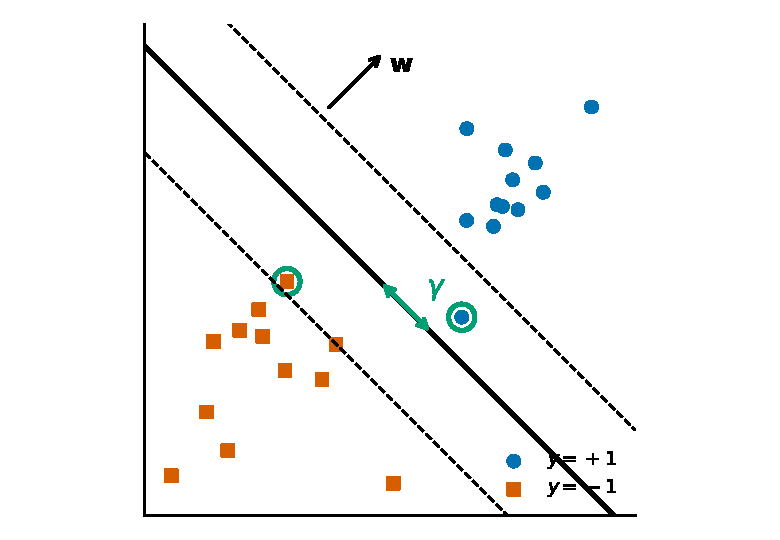
\includegraphics[height=0.36\textheight]{fig_margin.pdf}
\end{center}
\end{frame}

\begin{frame}{The Perceptron Algorithm (Rosenblatt, 1958)}\small
\begin{algorithm}[H]
\SetAlgoLined
\KwIn{$\{(\vx_i,y_i)\}_{i=1}^N$ with $y_i\in\{-1,+1\}$; $\vx_i$ augmented with a constant 1}
$\vw\gets\vzero$\;
\Repeat{no mistakes in a full pass}{
  \For{$i=1,\dots,N$}{
    \If{$y_i\,\vw\T\vx_i\le0$ \tcp*{mistake}}{
      $\vw\gets\vw+y_i\vx_i$\;
    }
  }
}
\KwOut{$\vw$}
\end{algorithm}
\vspace{4pt}
A mistake on $(\vx_i,y_i)$ moves $\vw$ toward $y_i\vx_i$. After the update,
\[
y_i\,(\vw+y_i\vx_i)\T\vx_i=y_i\vw\T\vx_i+\norm{\vx_i}^2 ,
\]
so the score on that example increases by $\norm{\vx_i}^2$. It need not become correct in one step.
\end{frame}

\begin{frame}{Numerical Example: Four Points, Seven Mistakes}\footnotesize
Augmented inputs $\tilde\vx=(x_1,x_2,1)$, visited in the order shown, $\vw^{(0)}=\vzero$.
A score of exactly $0$ counts as a mistake.
\begin{center}
\begin{tabular}{cccrcl}
\toprule
pass & $\tilde\vx$ & $y$ & $\vw\T\tilde\vx$ & mistake? & new $\vw$ \\
\midrule
1 & $(1,1,1)$ & $-1$ & $0$ & yes & $(-1,-1,-1)$ \\
1 & $(3,3,1)$ & $+1$ & $-7$ & yes & $(2,2,0)$ \\
1 & $(0,2,1)$ & $-1$ & $4$ & yes & $(2,0,-1)$ \\
1 & $(4,1,1)$ & $+1$ & $7$ & no & \\
2 & $(1,1,1)$ & $-1$ & $1$ & yes & $(1,-1,-2)$ \\
2 & $(3,3,1)$ & $+1$ & $-2$ & yes & $(4,2,-1)$ \\
2 & $(0,2,1)$ & $-1$ & $3$ & yes & $(4,0,-2)$ \\
2 & $(4,1,1)$ & $+1$ & $14$ & no & \\
3 & $(1,1,1)$ & $-1$ & $2$ & yes & $(3,-1,-3)$ \\
3 & $(3,3,1),(0,2,1),(4,1,1)$ & & $3,\,-5,\,8$ & no & \\
4 & all four & & $-1,\,3,\,-5,\,8$ & no & converged \\
\bottomrule
\end{tabular}
\end{center}
Final separator: $3x_1-x_2-3=0$. \ Seven updates. \ $R^2=\max_i\norm{\tilde\vx_i}^2=19$.
% verify: L2.perceptron_trace
\end{frame}

\begin{frame}{Numerical Example: The Picture}
\begin{center}
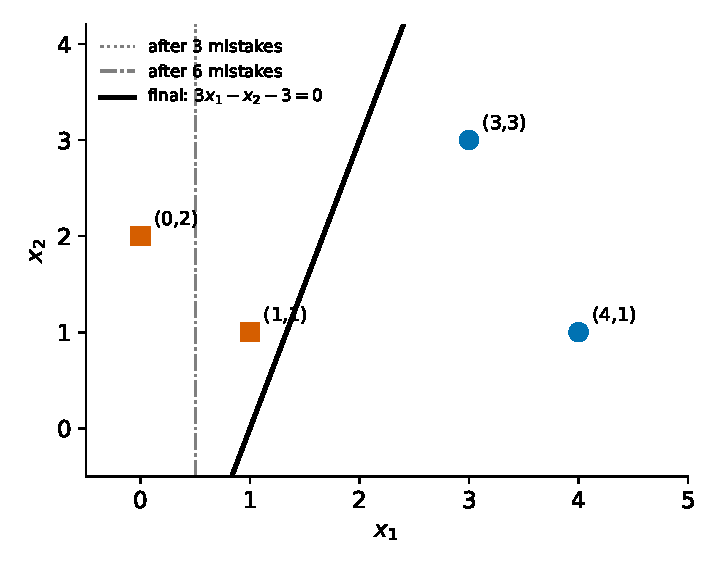
\includegraphics[height=0.72\textheight]{fig_perceptron.pdf}
\end{center}
\end{frame}

\begin{frame}{The Perceptron Mistake Bound (Novikoff, 1962)}
\begin{claim}{Theorem}
Suppose $\norm{\vx_i}\le R$ for all $i$, and there exists $\vw^\star$ with $\norm{\vw^\star}=1$ and
$y_i\,\vw^{\star\top}\vx_i\ge\gamma>0$ for all $i$ (the data are separable with margin $\gamma$).
Then the perceptron makes at most
\[
\frac{R^2}{\gamma^2}
\]
mistakes, regardless of the order in which examples are presented, and regardless of $N$.
\end{claim}
\vspace{6pt}
The proof tracks two quantities across mistakes: how much $\vw$ aligns with $\vw^\star$ (grows at least
linearly), and how long $\vw$ is (grows at most like a square root). They cannot both hold forever.
\end{frame}

\begin{frame}{Mistake Bound: Proof}\footnotesize
Let $\vw_k$ be the weight vector after the $k$-th mistake, $\vw_0=\vzero$, and let the $k$-th mistake be on $(\vx,y)$.
\begin{derivation}{Lower bound: alignment with $\vw^\star$ grows by at least $\gamma$ per mistake}
\[
\vw^{\star\top}\vw_k=\vw^{\star\top}(\vw_{k-1}+y\vx)=\vw^{\star\top}\vw_{k-1}+\underbrace{y\,\vw^{\star\top}\vx}_{\ge\gamma}
\ \ge\ \vw^{\star\top}\vw_{k-1}+\gamma
\quad\Longrightarrow\quad \vw^{\star\top}\vw_k\ge k\gamma .
\]
\end{derivation}
\begin{derivation}{Upper bound: the norm grows by at most $R^2$ per mistake}
\[
\norm{\vw_k}^2=\norm{\vw_{k-1}+y\vx}^2=\norm{\vw_{k-1}}^2+2\underbrace{y\,\vw_{k-1}\T\vx}_{\le0\ \text{(a mistake)}}+\underbrace{y^2\norm{\vx}^2}_{\le R^2}
\le\norm{\vw_{k-1}}^2+R^2
\ \Rightarrow\ \norm{\vw_k}^2\le kR^2 .
\]
\end{derivation}
\begin{derivation}{Combine with Cauchy--Schwarz}
\[
k\gamma\ \le\ \vw^{\star\top}\vw_k\ \le\ \norm{\vw^\star}\,\norm{\vw_k}=\norm{\vw_k}\ \le\ \sqrt{k}\,R
\qquad\Longrightarrow\qquad k\le\frac{R^2}{\gamma^2}.\qquad\qed
\]
\end{derivation}
\end{frame}

\begin{frame}{Reading the Bound}
\begin{itemize}
  \item The bound does not depend on $N$ or on the dimension $p$. It depends on the geometry only:
        how spread out the data are ($R$) relative to how separable they are ($\gamma$).
  \item It is a bound on \emph{mistakes}, not on passes. Correct examples cost nothing.
  \item It says nothing about which separator you end up with --- only that you end up with one.
        Different orders give different $\vw$. The SVM (next section) picks a canonical one.
\end{itemize}
\begin{caution}
If the data are not separable, the perceptron never terminates: it cycles forever. In practice one runs
a fixed number of epochs and keeps the $\vw$ with the best validation error --- an early-stopping rule.
\end{caution}
\begin{keypoint}
The perceptron update is SGD with $\eta=1$ on the \emph{perceptron loss} $\max(0,-y\vw\T\vx)$, whose
subgradient at a mistake is $-y\vx$. This loss is convex but has a trivial minimizer ($\vw=\vzero$),
which is why the algorithm is defined by its updates rather than by its objective.
\end{keypoint}
\end{frame}

% =============================================================================
\sectionframe{Support Vector Machines}
% =============================================================================

\begin{frame}{Which Separator?}
When data are separable, infinitely many hyperplanes achieve zero training error.
\begin{block}{Maximum-margin principle}
Choose the hyperplane whose geometric margin $\gamma=\min_i\gamma_i$ is largest.
\end{block}
Two reasons:
\begin{itemize}
  \item Robustness: the classifier's predictions on the training set survive the largest perturbation of the inputs.
  \item Generalization: bounds on test error for linear classifiers scale with $R^2/\gamma^2$ --- the same
        quantity as the perceptron's mistake bound. A large margin is evidence of a simple problem.
\end{itemize}
\vspace{4pt}
The maximizing hyperplane is unique, and it is determined by the few points that attain the minimum
margin --- the \textbf{support vectors}.
\end{frame}

\begin{frame}{From Margin to a Quadratic Program}\small
\begin{derivation}{Fix the scale, then the objective becomes $\norm\vw$}
Maximize $\gamma$ subject to every point having margin at least $\gamma$:
\[
\max_{\vw,b,\gamma}\ \gamma\quad\text{s.t.}\quad\frac{y_i(\vw\T\vx_i+b)}{\norm\vw}\ge\gamma\ \ \forall i .
\]
The constraints are invariant to rescaling $(\vw,b)$. Use that freedom to impose $\min_i y_i(\vw\T\vx_i+b)=1$.
Then $\gamma=1/\norm\vw$, and maximizing $1/\norm\vw$ is minimizing $\norm\vw$, or equivalently $\tfrac12\norm\vw^2$:
\[
\boxed{\ \min_{\vw,b}\ \frac12\norm{\vw}^2\quad\text{s.t.}\quad y_i(\vw\T\vx_i+b)\ge1\ \ \forall i\ }
\]
\end{derivation}
\begin{itemize}
  \item A convex quadratic objective with linear inequality constraints: a \textbf{quadratic program}.
        Unique solution, solvable by off-the-shelf methods.
  \item The constraint $y_i(\vw\T\vx_i+b)\ge1$ is the \emph{functional} margin; the geometric margin is $1/\norm\vw$.
\end{itemize}
\end{frame}

\begin{frame}{The Lagrangian and the Support Vectors}\footnotesize
Introduce multipliers $\alpha_i\ge0$ for the constraints:
\[
\Lcal(\vw,b,\valpha)=\frac12\norm\vw^2-\sum_{i=1}^N\alpha_i\bigl[y_i(\vw\T\vx_i+b)-1\bigr].
\]
\begin{derivation}{Stationarity in $\vw$ and $b$}
\[
\nabla_{\vw}\Lcal=\vw-\sum_i\alpha_iy_i\vx_i=\vzero\ \Rightarrow\ \boxed{\vw=\sum_{i=1}^N\alpha_iy_i\vx_i},
\qquad
\frac{\partial\Lcal}{\partial b}=-\sum_i\alpha_iy_i=0\ \Rightarrow\ \sum_i\alpha_iy_i=0 .
\]
\end{derivation}
\begin{derivation}{Complementary slackness}
At the optimum, $\alpha_i\bigl[y_i(\vw\T\vx_i+b)-1\bigr]=0$ for every $i$. So either $\alpha_i=0$, or the constraint
is tight: $y_i(\vw\T\vx_i+b)=1$, i.e.\ $\vx_i$ sits exactly on the margin.
\end{derivation}
\begin{keypoint}
$\vw$ is a linear combination of the training points, with nonzero weight only on those on the margin.
Delete any other point and the solution does not change.
\end{keypoint}
\end{frame}

\begin{frame}{Soft Margin}\small
Real data are not separable. Allow each constraint to be violated by a slack $\xi_i\ge0$, and pay for it:
\[
\min_{\vw,b,\vxi}\ \frac12\norm\vw^2+C\sum_{i=1}^N\xi_i
\quad\text{s.t.}\quad y_i(\vw\T\vx_i+b)\ge1-\xi_i,\ \ \xi_i\ge0 .
\]
\begin{derivation}{Eliminate the slacks: the constraint problem is an unconstrained loss}
For fixed $(\vw,b)$, the optimal $\xi_i$ is the smallest feasible one:
$\xi_i=\max\bigl(0,\,1-y_i(\vw\T\vx_i+b)\bigr)$. Substituting,
\[
\boxed{\ \min_{\vw,b}\ \frac12\norm\vw^2+C\sum_{i=1}^N\max\bigl(0,\,1-y_i(\vw\T\vx_i+b)\bigr)\ }
\]
\end{derivation}
This is empirical risk minimization with the \textbf{hinge loss} $\ell_{\text{hinge}}(y,f)=\max(0,1-yf)$
and an $\ell_2$ penalty on $\vw$ --- the recipe of Lecture 1 again, plus the regularizer of Lecture 3.
$C$ trades margin width against training violations.
\end{frame}

\begin{frame}{The Hinge Loss}
\begin{claim}{Hinge is a convex upper bound on 0/1}
For $y\in\{-1,+1\}$ and score $f$, let $m=yf$ (the functional margin).
\begin{itemize}
  \item $\ell_{0/1}=\ind{m\le0}$ and $\ell_{\text{hinge}}=\max(0,1-m)$.
  \item If $m\le0$: $1-m\ge1=\ell_{0/1}$. If $m>0$: $\ell_{\text{hinge}}\ge0=\ell_{0/1}$. So $\ell_{\text{hinge}}\ge\ell_{0/1}$ always.
  \item $\max(0,1-m)$ is the maximum of two affine functions of $m$, hence convex in $m$, hence convex in $\vw$.
\end{itemize}
\end{claim}
\end{frame}

\begin{frame}{The Hinge Loss: Subgradient}
\begin{derivation}{Subgradient}
$\ell_{\text{hinge}}$ is not differentiable at $m=1$. A subgradient with respect to $\vw$ is
\[
\partial_{\vw}\,\ell_{\text{hinge}}=\begin{cases}-y\vx & \text{if } y(\vw\T\vx+b)<1,\\ \vzero & \text{if } y(\vw\T\vx+b)>1,\end{cases}
\]
and anything in between at equality. SGD with this subgradient is the standard large-scale SVM solver.
\end{derivation}
\begin{keypoint}
Minimizing an upper bound on the 0/1 risk controls the 0/1 risk. That is the whole logic of surrogate losses.
\end{keypoint}
\end{frame}

% =============================================================================
\sectionframe{Logistic Regression}
% =============================================================================

\begin{frame}{Modelling a Probability}
Instead of a hard label, model $p(\vx)=\Prob(Y=1\mid\vx)$ for $y\in\{0,1\}$. A linear function is the wrong
object: $\vx\T\vbeta$ ranges over $\R$. Pass it through the \textbf{logistic (sigmoid) function}:
\[
\sigma(z)=\frac{1}{1+e^{-z}}=\frac{e^z}{1+e^z},\qquad
p(\vx)=\sigma(\vx\T\vbeta).
\]
\begin{columns}[T]
\begin{column}{0.58\textwidth}\footnotesize
\begin{derivation}{Log-odds are linear}
\[
\frac{p}{1-p}=\frac{e^z/(1+e^z)}{1/(1+e^z)}=e^z
\ \Rightarrow\ \log\frac{p(\vx)}{1-p(\vx)}=\vx\T\vbeta .
\]
\end{derivation}
A unit increase in $x_j$ multiplies the odds by $e^{\beta_j}$.
\end{column}
\begin{column}{0.38\textwidth}
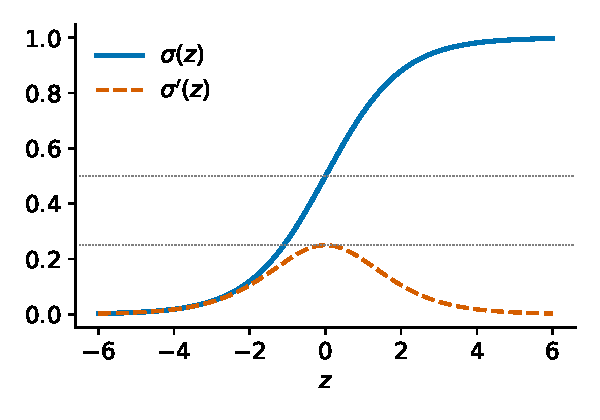
\includegraphics[width=\textwidth]{fig_sigmoid.pdf}
\end{column}
\end{columns}
\end{frame}

\begin{frame}{The Derivative of the Sigmoid}
\begin{derivation}{$\sigma'(z)=\sigma(z)\bigl(1-\sigma(z)\bigr)$}
\[
\sigma'(z)=\frac{d}{dz}(1+e^{-z})^{-1}=-(1+e^{-z})^{-2}\cdot(-e^{-z})=\frac{e^{-z}}{(1+e^{-z})^2}
=\underbrace{\frac{1}{1+e^{-z}}}_{\sigma(z)}\cdot\underbrace{\frac{e^{-z}}{1+e^{-z}}}_{1-\sigma(z)} .
\]
\end{derivation}
Also useful: $1-\sigma(z)=\sigma(-z)$, and $\sigma'(z)\le\tfrac14$ with equality at $z=0$.
\vspace{6pt}

The identity $\sigma'=\sigma(1-\sigma)$ is the reason every gradient in this section is short. It reappears
in ML II as the source of the vanishing-gradient problem.
\end{frame}

\begin{frame}{Likelihood}\small
The model says $Y_i\mid\vx_i\sim\text{Bernoulli}(p_i)$ with $p_i=\sigma(\vx_i\T\vbeta)$, independently. The
probability of the observed labels is
\[
L(\vbeta)=\prod_{i=1}^N p_i^{\,y_i}(1-p_i)^{1-y_i}.
\]
\begin{derivation}{Log-likelihood}
\begin{align*}
\ell(\vbeta)=\log L(\vbeta)&=\sum_{i=1}^N\Bigl[y_i\log p_i+(1-y_i)\log(1-p_i)\Bigr]\\
&=\sum_{i=1}^N\Bigl[y_i\log\frac{p_i}{1-p_i}+\log(1-p_i)\Bigr]
=\sum_{i=1}^N\Bigl[y_i\,\vx_i\T\vbeta-\log\bigl(1+e^{\vx_i\T\vbeta}\bigr)\Bigr],
\end{align*}
using $\log\frac{p}{1-p}=\vx\T\vbeta$ and $1-p_i=\frac1{1+e^{\vx_i\T\vbeta}}$.
\end{derivation}
The MLE is $\hat\vbeta=\argmax_{\vbeta}\ell(\vbeta)$. Equivalently we minimize $-\ell$, the \textbf{log loss}.
\end{frame}

\begin{frame}{The Gradient}
\begin{derivation}{$\nabla_{\vbeta}\,\ell(\vbeta)=\sum_{i=1}^N(y_i-p_i)\,\vx_i$}
Differentiate term by term, with $z_i=\vx_i\T\vbeta$ and $\nabla_{\vbeta} z_i=\vx_i$:
\begin{align*}
\nabla_{\vbeta}\Bigl[y_iz_i-\log(1+e^{z_i})\Bigr]
&=y_i\vx_i-\frac{e^{z_i}}{1+e^{z_i}}\,\vx_i
=y_i\vx_i-\sigma(z_i)\,\vx_i=(y_i-p_i)\,\vx_i .
\end{align*}
\end{derivation}
\begin{itemize}
  \item Same shape as least squares: residual $(y_i-p_i)$ times input. The residual is now a difference
        of a label and a probability.
  \item Setting the gradient to zero gives the \textbf{score equations} $\sum_i(y_i-p_i)\vx_i=\vzero$:
        nonlinear in $\vbeta$ through $p_i$, hence no closed form.
  \item With an intercept, the first score equation reads $\sum_iy_i=\sum_ip_i$: the fitted probabilities
        sum to the observed count. (Compare: least-squares residuals sum to zero.)
\end{itemize}
\end{frame}

\begin{frame}{The Hessian, and Concavity}\small
\begin{derivation}{$\nabla^2_{\vbeta}\,\ell(\vbeta)=-\sum_{i=1}^Np_i(1-p_i)\,\vx_i\vx_i\T$}
Differentiate the gradient once more. Only $p_i=\sigma(\vx_i\T\vbeta)$ depends on $\vbeta$:
\[
\nabla_{\vbeta}\bigl[(y_i-p_i)\vx_i\bigr]=-\vx_i\bigl(\nabla_{\vbeta} p_i\bigr)\T
=-\vx_i\bigl(\sigma'(z_i)\,\vx_i\bigr)\T=-p_i(1-p_i)\,\vx_i\vx_i\T .
\]
\end{derivation}
\begin{claim}{The Hessian is negative semidefinite, so $\ell$ is concave}
For any $\vv$,
\[
\vv\T\nabla^2\ell\,\vv=-\sum_{i=1}^Np_i(1-p_i)\underbrace{(\vv\T\vx_i)^2}_{\ge0}\ \le\ 0,
\]
since $p_i(1-p_i)\in(0,\tfrac14]$. Strictly negative when $\vX$ has full column rank.
\end{claim}
\begin{keypoint}
Concave log-likelihood $\Rightarrow$ convex log loss $\Rightarrow$ every stationary point is the global MLE, and
gradient descent (with $L=\tfrac14\lambda_{\max}(\vX\T\vX)$) converges at the $O(1/t)$ rate of \S1.
\end{keypoint}
\end{frame}

\begin{frame}{Newton's Method}\small
Gradient descent uses the first-order Taylor expansion. Newton's method uses the second:
\begin{derivation}{Maximize the quadratic model}
\[
\ell(\vbeta+\vdelta)\approx\ell(\vbeta)+\nabla\ell(\vbeta)\T\vdelta+\frac12\vdelta\T\nabla^2\ell(\vbeta)\,\vdelta .
\]
Setting the $\vdelta$-gradient to zero: $\nabla\ell+\nabla^2\ell\,\vdelta=\vzero$, so
\[
\vbeta^{(t+1)}=\vbeta^{(t)}-\bigl[\nabla^2\ell(\vbeta^{(t)})\bigr]\inv\nabla\ell(\vbeta^{(t)}).
\]
\end{derivation}
\begin{itemize}
  \item The Hessian is invertible (negative definite) whenever $\vX$ has full column rank, so the step is well defined.
  \item Near the optimum, Newton converges \emph{quadratically}: the number of correct digits doubles per iteration.
        Five to ten iterations typically suffice.
  \item Cost per iteration $O(Np^2+p^3)$ --- the same as one least-squares solve. For $p$ in the thousands, use
        gradient methods instead.
\end{itemize}
\end{frame}

\begin{frame}{Newton $=$ Iteratively Reweighted Least Squares}\small
Write $\vp=(p_1,\dots,p_N)\T$ and $\vW=\diag\bigl(p_i(1-p_i)\bigr)$. In matrix form,
\[
\nabla\ell=\vX\T(\vy-\vp),\qquad \nabla^2\ell=-\vX\T\vW\vX .
\]
\begin{derivation}{Rewrite the Newton step as a weighted least-squares solve}
\begin{align*}
\vbeta^{(t+1)}&=\vbeta^{(t)}+(\vX\T\vW\vX)\inv\vX\T(\vy-\vp)\\
&=(\vX\T\vW\vX)\inv\Bigl[\vX\T\vW\vX\vbeta^{(t)}+\vX\T(\vy-\vp)\Bigr]
=(\vX\T\vW\vX)\inv\vX\T\vW\underbrace{\Bigl[\vX\vbeta^{(t)}+\vW\inv(\vy-\vp)\Bigr]}_{\vz}\\
&=\boxed{(\vX\T\vW\vX)\inv\vX\T\vW\vz}
\end{align*}
\end{derivation}
Each Newton step is the solution of $\min_{\vbeta}\sum_iW_{ii}(z_i-\vx_i\T\vbeta)^2$: a least-squares problem on the
\emph{working response} $\vz$, with weights that are largest for uncertain points ($p_i\approx\tfrac12$).
Weights and working response are recomputed each iteration --- hence \textbf{IRLS}.
\end{frame}

\begin{frame}{Numerical Example: One IRLS Step}\footnotesize
Three points with intercept: $\vx_i=(1,x_i)$, $x=(-1,0,1)$, $y=(0,0,1)$. Start at $\vbeta^{(0)}=\vzero$.
\begin{derivation}{Step}
At $\vbeta=\vzero$ every $p_i=\sigma(0)=\tfrac12$, so $\vW=\tfrac14\vI$ and
$\vz=\vX\vzero+\vW\inv(\vy-\vp)=4(\vy-\tfrac12\vone)=(-2,-2,2)\T$.
\[
\vX\T\vW\vX=\tfrac14\begin{pmatrix}3&0\\0&2\end{pmatrix},\qquad
\vX\T\vW\vz=\tfrac14\begin{pmatrix}-2-2+2\\ 2+0+2\end{pmatrix}=\begin{pmatrix}-\tfrac12\\1\end{pmatrix},\qquad
\vbeta^{(1)}=\begin{pmatrix}4/3&0\\0&2\end{pmatrix}\begin{pmatrix}-\tfrac12\\1\end{pmatrix}=\begin{pmatrix}-\tfrac23\\2\end{pmatrix}.
\]
\end{derivation}
Check against the raw Newton form: $\nabla\ell(\vzero)=\sum_i(y_i-\tfrac12)\vx_i=(-\tfrac12,\,1)\T$ and
$-\nabla^2\ell(\vzero)=\tfrac14\vX\T\vX$, so $\vbeta^{(1)}=\vzero+(\tfrac14\vX\T\vX)\inv(-\tfrac12,1)\T=(-\tfrac23,\,2)\T$. Same answer.
\vspace{4pt}

After the step, $p=\sigma(-\tfrac23-2,\,-\tfrac23,\,-\tfrac23+2)\approx(0.065,\,0.339,\,0.791)$; the score equations are not yet zero,
and three more steps bring $\vbeta$ to convergence.
% verify: L2.irls_step
\end{frame}

\begin{frame}{When the MLE Does Not Exist}
\begin{caution}
If the training data are linearly separable, logistic regression has \textbf{no} maximum-likelihood
estimate.
\end{caution}
\begin{derivation}{Why}
Let $\vbeta_0$ separate the data: $y_i=1\Rightarrow\vx_i\T\vbeta_0>0$ and $y_i=0\Rightarrow\vx_i\T\vbeta_0<0$.
Consider $\vbeta=c\,\vbeta_0$ with $c\to\infty$. Then $p_i\to1$ for every $y_i=1$ and $p_i\to0$ for every
$y_i=0$, so each term of $\ell$ increases toward $0$ and $\ell(c\vbeta_0)\uparrow0=\sup\ell$.
The supremum is approached only as $\norm\vbeta\to\infty$; it is never attained.
\end{derivation}
\begin{itemize}
  \item Numerically: coefficients blow up, fitted probabilities saturate at $0$ and $1$, standard errors are meaningless.
  \item The fix is to penalize $\norm\vbeta$ --- Lecture 3. Regularized logistic regression always has a unique solution.
  \item Contrast with the perceptron, for which separable data are the \emph{good} case.
\end{itemize}
\end{frame}

\begin{frame}{Asymptotics}
Under standard regularity conditions the MLE is consistent and asymptotically normal:
\[
\sqrt N\,(\hat\vbeta-\vbeta_0)\ \xrightarrow{d}\ \Ncal\bigl(\vzero,\ \mathcal I(\vbeta_0)\inv\bigr),\qquad
\mathcal I(\vbeta_0)=\E\bigl[p(\vx)(1-p(\vx))\,\vx\vx\T\bigr].
\]
\begin{itemize}
  \item $\mathcal I$ is the Fisher information --- the negative expected Hessian per observation. Its sample
        version is $\tfrac1N\vX\T\vW\vX$, the matrix IRLS inverts at convergence.
  \item Standard errors are the square roots of the diagonal of $(\vX\T\hat\vW\vX)\inv$; Wald, score and
        likelihood-ratio tests follow.
  \item The parallel with least squares is exact: there, $\Var(\hat\vbeta)=\sigma^2(\vX\T\vX)\inv$; here,
        $\Var(\hat\vbeta)\approx(\vX\T\vW\vX)\inv$, with the variance of $Y_i$ absorbed into $W_{ii}=p_i(1-p_i)$.
\end{itemize}
\end{frame}

% =============================================================================
\sectionframe{The Loss Functions, Side by Side}
% =============================================================================

\begin{frame}{One Axis: The Margin}
Convert logistic regression to $y\in\{-1,+1\}$: with $\tilde y=2y-1$, one checks
$-\log p_i^{y_i}(1-p_i)^{1-y_i}=\log\bigl(1+e^{-\tilde y_i\,\vx_i\T\vbeta}\bigr)$.
Every loss today is a function of the margin $m=yf(\vx)$:
\begin{center}
\begin{tabular}{lll}
\toprule
Loss & $\ell(m)$ & Minimizer, and what it estimates \\
\midrule
0/1 & $\ind{m\le0}$ & the Bayes classifier; intractable \\
Perceptron & $\max(0,-m)$ & any separator; degenerate on non-separable data \\
Hinge & $\max(0,1-m)$ & max-margin separator; a \emph{classifier}, not a probability \\
Log & $\log(1+e^{-m})$ & $\log\frac{P(y=1\mid\vx)}{P(y=-1\mid\vx)}$; a calibrated probability \\
Squared & $(1-m)^2$ & penalizes $m>1$ too; wrong shape for classification \\
\bottomrule
\end{tabular}
\end{center}
\end{frame}

\begin{frame}{The Picture}
\begin{center}
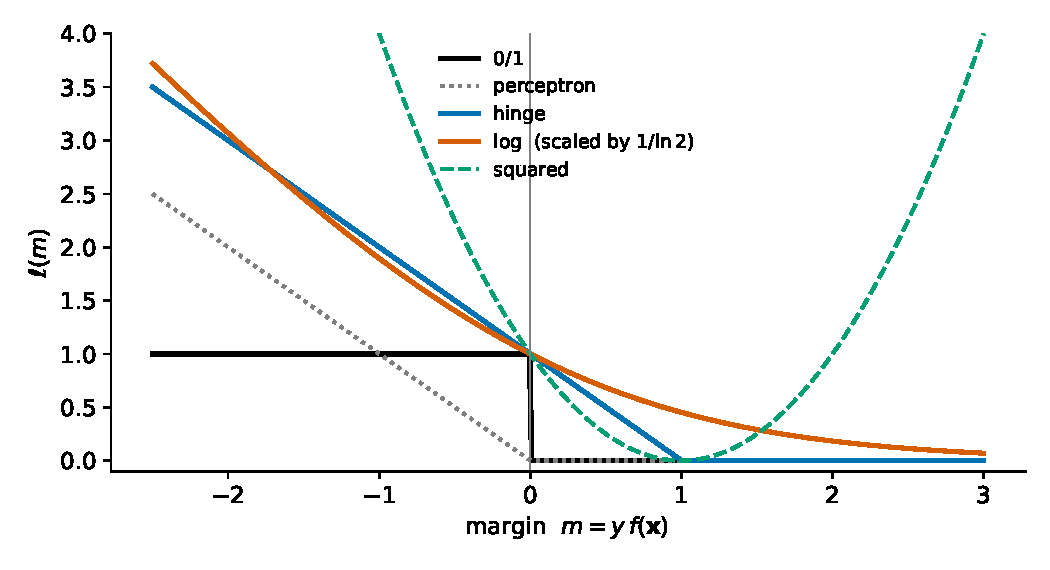
\includegraphics[height=0.72\textheight]{fig_losses.pdf}
\end{center}
\vspace{-6pt}
Hinge and log both upper-bound 0/1, are convex, and vanish (or nearly) for confident correct
predictions. Squared loss rises again on the right: it punishes being \emph{too} right.
\end{frame}

\begin{frame}{What We Proved Today}
\begin{enumerate}
  \item Descent lemma for $L$-smooth $f$; with $\eta\le1/L$, $f(\vx_{t+1})\le f(\vx_t)-\tfrac\eta2\norm{\nabla f}^2$.
  \item Convex $+$ smooth $\Rightarrow$ $f(\vx_t)-f^\star\le L\norm{\vx_0-\vx^\star}^2/(2t)$.
  \item Perceptron: at most $R^2/\gamma^2$ mistakes on data separable with margin $\gamma$ (Novikoff).
  \item Max margin $\Leftrightarrow$ $\min\tfrac12\norm\vw^2$ s.t.\ $y_i(\vw\T\vx_i+b)\ge1$; $\vw=\sum_i\alpha_iy_i\vx_i$ with
        $\alpha_i\ne0$ only on support vectors; soft margin $\Leftrightarrow$ hinge loss $+$ $\ell_2$ penalty.
  \item Logistic regression: $\nabla\ell=\vX\T(\vy-\vp)$, $\nabla^2\ell=-\vX\T\vW\vX\preceq0$; Newton $=$ IRLS;
        no MLE on separable data.
\end{enumerate}
\end{frame}

\begin{frame}{Next}
\textbf{Lecture 3 (Monday)} --- ridge and lasso: closed forms, shrinkage in the SVD basis, why $\ell_1$
gives exact zeros; then evaluation: precision, recall, ROC, and cost-sensitive thresholds.
\vspace{8pt}

\textbf{Lab 2 (Wednesday, Rodrigo)} --- ridge vs.\ lasso paths, cross-validated $\lambda$, and the
separable-data failure of unregularized logistic regression, seen live.
\vspace{8pt}

\textbf{Reading} --- \emph{ESL} \S4.4 (logistic regression), \S4.5 (separating hyperplanes),
\S12.1--12.2 (SVM). Novikoff (1962) is two pages and worth reading in the original.
\end{frame}

\end{document}
